\documentclass[a4paper]{report}

\usepackage{geometry}

\usepackage{caption}
\usepackage{amsmath}

\captionsetup[table]{position=bottom}

%\usepackage[cm]{fullpage}

% some very useful LaTeX packages include:

%\usepackage{cite}      % Written by Donald Arseneau
                        % V1.6 and later of IEEEtran pre-defines the format
                        % of the cite.sty package \cite{} output to follow
                        % that of IEEE. Loading the cite package will
                        % result in citation numbers being automatically
                        % sorted and properly "ranged". i.e.,
                        % [1], [9], [2], [7], [5], [6]
                        % (without using cite.sty)
                        % will become:
                        % [1], [2], [5]--[7], [9] (using cite.sty)
                        % cite.sty's \cite will automatically add leading
                        % space, if needed. Use cite.sty's noadjust option
                        % (cite.sty V3.8 and later) if you want to turn this
                        % off. cite.sty is already installed on most LaTeX
                        % systems. The latest version can be obtained at:
                        % http://www.ctan.org/tex-archive/macros/latex/contrib/supported/cite/
\usepackage[inline]{enumitem}

\usepackage{graphicx}   % Written by David Carlisle and Sebastian Rahtz
                        % Required if you want graphics, photos, etc.
                        % graphicx.sty is already installed on most LaTeX
                        % systems. The latest version and documentation can
                        % be obtained at:
                        % http://www.ctan.org/tex-archive/macros/latex/required/graphics/
                        % Another good source of documentation is "Using
                        % Imported Graphics in LaTeX2e" by Keith Reckdahl
                        % which can be found as esplatex.ps and epslatex.pdf
                        % at: http://www.ctan.org/tex-archive/info/

%\usepackage{psfrag}    % Written by Craig Barratt, Michael C. Grant,
                        % and David Carlisle
                        % This package allows you to substitute LaTeX
                        % commands for text in imported EPS graphic files.
                        % In this way, LaTeX symbols can be placed into
                        % graphics that have been generated by other
                        % applications. You must use latex->dvips->ps2pdf
                        % workflow (not direct pdf output from pdflatex) if
                        % you wish to use this capability because it works
                        % via some PostScript tricks. Alternatively, the
                        % graphics could be processed as separate files via
                        % psfrag and dvips, then converted to PDF for
                        % inclusion in the main file which uses pdflatex.
                        % Docs are in "The PSfrag System" by Michael C. Grant
                        % and David Carlisle. There is also some information
                        % about using psfrag in "Using Imported Graphics in
                        % LaTeX2e" by Keith Reckdahl which documents the
                        % graphicx package (see above). The psfrag package
                        % and documentation can be obtained at:
                        % http://www.ctan.org/tex-archive/macros/latex/contrib/supported/psfrag/

%\usepackage{subfigure} % Written by Steven Douglas Cochran
                        % This package makes it easy to put subfigures
                        % in your figures. i.e., "figure 1a and 1b"
                        % Docs are in "Using Imported Graphics in LaTeX2e"
                        % by Keith Reckdahl which also documents the graphicx
                        % package (see above). subfigure.sty is already
                        % installed on most LaTeX systems. The latest version
                        % and documentation can be obtained at:
                        % http://www.ctan.org/tex-archive/macros/latex/contrib/supported/subfigure/

\usepackage{url}        % Written by Donald Arseneau
                        % Provides better support for handling and breaking
                        % URLs. url.sty is already installed on most LaTeX
                        % systems. The latest version can be obtained at:
                        % http://www.ctan.org/tex-archive/macros/latex/contrib/other/misc/
                        % Read the url.sty source comments for usage information.

%\usepackage{stfloats}  % Written by Sigitas Tolusis
                        % Gives LaTeX2e the ability to do double column
                        % floats at the bottom of the page as well as the top.
                        % (e.g., "\begin{figure*}[!b]" is not normally
                        % possible in LaTeX2e). This is an invasive package
                        % which rewrites many portions of the LaTeX2e output
                        % routines. It may not work with other packages that
                        % modify the LaTeX2e output routine and/or with other
                        % versions of LaTeX. The latest version and
                        % documentation can be obtained at:
                        % http://www.ctan.org/tex-archive/macros/latex/contrib/supported/sttools/
                        % Documentation is contained in the stfloats.sty
                        % comments as well as in the presfull.pdf file.
                        % Do not use the stfloats baselinefloat ability as
                        % IEEE does not allow \baselineskip to stretch.
                        % Authors submitting work to the IEEE should note
                        % that IEEE rarely uses double column equations and
                        % that authors should try to avoid such use.
                        % Do not be tempted to use the cuted.sty or
                        % midfloat.sty package (by the same author) as IEEE
                        % does not format its papers in such ways.
\usepackage{amssymb}
\usepackage{amsmath}    % From the American Mathematical Society
                        % A popular package that provides many helpful commands
                        % for dealing with mathematics. Note that the AMSmath
                        % package sets \interdisplaylinepenalty to 10000 thus
                        % preventing page breaks from occurring within multiline
                        % equations. Use:
%\interdisplaylinepenalty=2500
                        % after loading amsmath to restore such page breaks
                        % as IEEEtran.cls normally does. amsmath.sty is already
                        % installed on most LaTeX systems. The latest version
                        % and documentation can be obtained at:
                        % http://www.ctan.org/tex-archive/macros/latex/required/amslatex/math/
\usepackage{latexsym}
\usepackage{amsthm}

\usepackage{verbatim}

\usepackage[utf8]{inputenc}
\usepackage[italian]{babel}

\usepackage[htt]{hyphenat}

\hyphenation{en-ter-crit-i-cal-sec-tion}
\hyphenation{ex-it-crit-i-cal-sec-tion}

\setcounter{secnumdepth}{4}

\setlength{\parindent}{0pt}

\usepackage{algorithm}
\usepackage{algpseudocode}
\algrenewcommand{\algorithmiccomment}[1]{$\left(\text{#1}\right)$}

\usepackage{color}

\definecolor{ideanumber}{rgb}{0.0,0.0,1.0}
\definecolor{ideacomment}{rgb}{0.5,0.5,0.5}
\definecolor{ideakeyword}{rgb}{0.0,0.0,0.5}
\definecolor{ideastring}{rgb}{0.0,0.5,0.0}

\usepackage{listings}
\lstset{frame=tb,
    language=Java,
    aboveskip=3mm,
    belowskip=3mm,
    showstringspaces=false,
    columns=flexible,
    basicstyle={\small\ttfamily},
    numbers=left,
    numbersep=2pt,                   % how far the line-numbers are from the code
    numberstyle=\tiny\color{ideacomment},
    keywordstyle=\color{ideakeyword},
    commentstyle=\color{ideacomment},
    stringstyle=\color{ideastring},
    breaklines=true,
    breakatwhitespace=true,
    tabsize=4
}

% Other popular packages for formatting tables and equations include:

%\usepackage{array}
% Frank Mittelbach's and David Carlisle's array.sty which improves the
% LaTeX2e array and tabular environments to provide better appearances and
% additional user controls. array.sty is already installed on most systems.
% The latest version and documentation can be obtained at:
% http://www.ctan.org/tex-archive/macros/latex/required/tools/

% V1.6 of IEEEtran contains the IEEEeqnarray family of commands that can
% be used to generate multiline equations as well as matrices, tables, etc.

% Also of notable interest:
% Scott Pakin's eqparbox package for creating (automatically sized) equal
% width boxes. Available:
% http://www.ctan.org/tex-archive/macros/latex/contrib/supported/eqparbox/

% *** Do not adjust lengths that control margins, column widths, etc. ***
% *** Do not use packages that alter fonts (such as pslatex).         ***
% There should be no need to do such things with IEEEtran.cls V1.6 and later.
\newcommand\textsup[1]{$^{\text{#1}}$}
\newcommand\textsub[1]{$_{\text{#1}}$}

% Define document title and author
\title{\Huge \bf
Assignment \#3
}
\author{
    Martina Magnani\\
    \texttt{martina.magnani8@studio.unibo.it}
    \and
    Nicola Piscaglia\\
    \texttt{nicola.piscaglia2@studio.unibo.it}
    \and
    Mattia Vandi\\
    \texttt{mattia.vandi@studio.unibo.it}
}
\date{}

% Your document starts here!
\begin{document}

\maketitle

\tableofcontents

\chapter{Esercizio 1 - Actor-based Game of Life}
\section{Analisi del problema}\label{analisi-del-problema-1}

L'obiettivo della consegna è implementare Implementare in Java o in Scala una versione ad attori del gioco \textit{``The Game of Life''}.\\
Il gioco consiste nel calcolare e visualizzare l'evoluzione della matrice di celle che caratterizza il gioco, come sequenza di fotogrammi (ognuno dei quali rappresenta lo stato del mondo).\\
Nella matrice, ogni cella può essere in uno dei due stati possibili, \textit{live} o \textit{dead}.\\
Dato lo stato $s\left(t\right)$ della matrice, lo stato $s\left(t + 1\right)$ si computa con le seguenti regole:

\begin{itemize}
\item
  una cella $m\left[i,j\right]$ che nello stato $s\left(t\right)$ è \textit{live} e ha zero o al più una cella vicina \textit{live} (e le altre \textit{dead}), nello stato $s\left(t + 1\right)$ diventa \textit{dead} (``muore di solitudine'')
\item
  una cella $m\left[i,j\right]$ che nello stato $s\left(t\right)$ è \textit{live} e ha quattro o più celle vicine \textit{live}, nello stato $s\left(t + 1\right)$ diventa \textit{dead} (``muore di sovrappopolamento'')
\item
  una cella $m\left[i,j\right]$ che nello stato $s\left(t\right)$ è \textit{live} e ha due o tre celle vicine \textit{live}, nello stato $s\left(t + 1\right)$ rimane \textit{live} (``sopravvive'')
\item
  una cella $m\left[i,j\right]$ che nello stato $s\left(t\right)$ è \textit{dead} e ha tre celle vicine \textit{live}, nello stato $s\left(t + 1\right)$ diventa \textit{live}
\end{itemize}
Il gioco deve presentare un'interfaccia grafica con pulsanti \texttt{start} e \texttt{stop} con cui si fa partire e fermare il gioco.
Ogni stato del gioco deve essere visualizzato, insieme al numero di celle nello stato \textit{live}.

\subsection{Requisiti del sistema}\label{requisiti-del-sistema-1}

\begin{itemize}
\item
  Il programma deve funzionare anche con matrici di dimensioni significative (ad es. 5000x5000);
\item
  Massimizzare il throughput, minimizzando il tempo di calcolo di ciascun fotogramma ed eventualmente anche della sequenza di fotogrammi;
\item
  Massimizzare la reattività della GUI;
\item
  Studiare e implementare meccanismi di coordinazione/sincronizzazione basati sullo scambio di messaggi.
\end{itemize}

\section{Descrizione della soluzione proposta}\label{descrizione-della-soluzione-proposta-1}

\subsection{Architettura del sistema}\label{architettura-del-sistema-1}

L'architettura del sistema è stata scomposta in tre livelli utilizzando il pattern Model View Presenter, a differenza della prima consegna l'aggiornamento della schermata utente e l'aggiornamento della scacchiera di gioco è completamente demandata ad un insieme di attori, di conseguenza vi sono tre moduli: il dominio applicativo, gli attori e l'interfaccia grafica:

\begin{itemize}
\item
  Nel primo livello vi è una rappresentazione object-oriented delle componenti del problema;
\item
  Nel secondo livello è stata incapsulata la logica di aggiornamento del gioco e dell'interfaccia utente;
\item
  Nel terzo livello viene organizzata l'interfaccia grafica che permette la visualizzazione del gioco e l'interazione con l'utente.
\end{itemize}

\subsection{Dinamica del sistema}\label{dinamica-del-sistema-1}
La dinamica del sistema è stata rappresentata ad alto livello con un diagramma di sequenza, adatto per mostrare in modo efficace lo scambio di messaggi tra le entità del sistema.

\begin{figure}[H]
    \centering
    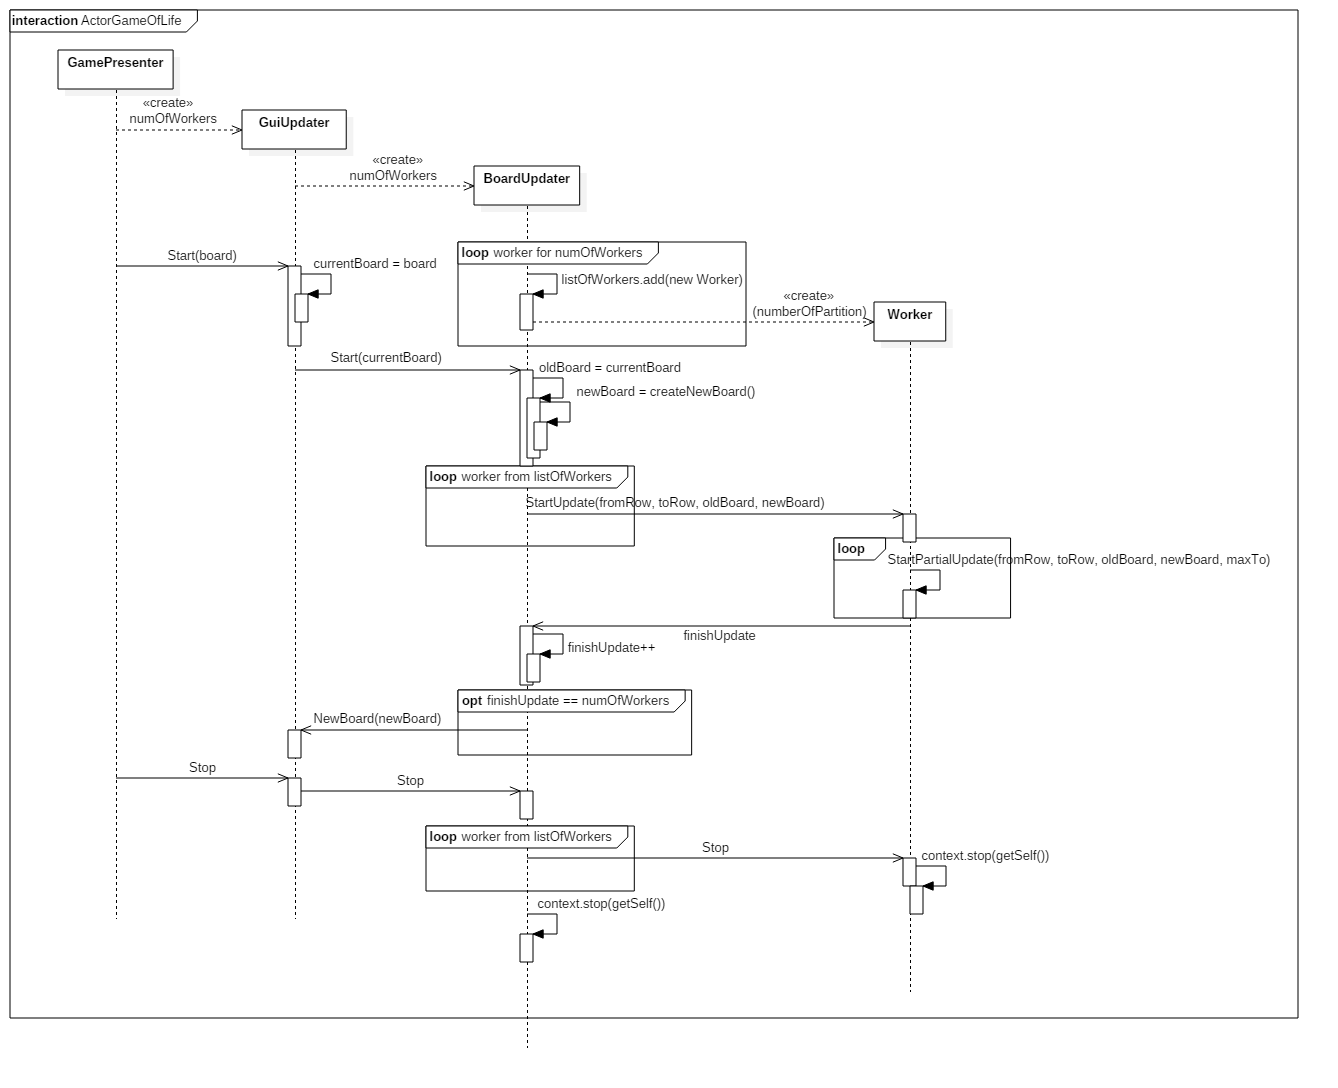
\includegraphics[width=\linewidth, height=\textheight, keepaspectratio]{res/ActorGameOfLife.png}
    \caption{Diagramma di sequenza che modella la dinamica della computazione dello stato di gioco}
    \label{fig:sequencediagram}
\end{figure}

\subsection{Implementazione}\label{implementazione-1}

\subsubsection{Dominio applicativo}\label{dominio-applicativo-1}

Abbiamo implementato il dominio applicativo attraverso due classi: \texttt{Cell} e \texttt{Board}.\\
L'enumerazione \texttt{Cell} rappresenta lo stato di una cella della scacchiera che può essere \textit{live} o \textit{dead}.
La classe \texttt{Board} rappresenta la scacchiera di gioco. Questa è caratterizzata da un'\textit{altezza} e una \textit{larghezza} variabili e dalla possibilità di recuperare/impostare lo stato di una cella date le coordinate $x$ e $y$.

\subsubsection{Attori}\label{attori}

Abbiamo implementato un attore \texttt{BoardUpdater} che si occupa dell'aggiornamento della scacchiera di gioco.

Dell'attore \texttt{BoardUpdater} è possibile configurare il numero di \texttt{Worker} che verranno utilizzati per aggiornare la schermata di gioco (ognuno dei quali verrà tradotto in un nuovo attore).

\begin{itemize}
    \item Il messaggio \texttt{StartUpdate}, inviato dal \texttt{BoardUpdater}, informa ogni \texttt{Worker} della porzione di scacchiera di gioco che dovrà aggiornare.
    \item Il messaggio \texttt{StartPartialUpdate}, inviato da un \texttt{Worker} sé stesso, informa sé stesso sulla porzione di scacchiera di gioco da aggiornare prima di passare alla successiva. Tale strategia consente ad un attore di rimanere reattivo ai messaggi ricevuti da altri attori.
    \item Il messaggio \texttt{FinishedPartialUpdate}, inviato da un \texttt{Worker} a sé stesso, informa sé stesso che un aggiornamento parziale è terminato. Se l'aggiornamento parziale completato è l'ultimo allora informa sé stesso che può informare il \texttt{BoardUpdater} che l'aggiornamento assegnato al \texttt{Worker} è terminato, altrimenti l'attore informa sé stesso sulla prossima porzione di scacchiera da aggiornare.
    \item Il messagio \texttt{FinishedUpdate}, inviato ad un \texttt{Worker}, informa il \texttt{BoardUpdater} che l'aggiornamento assegnato ad un \texttt{Worker} è termianto. Se l'aggiornamento terminato è anche l'ultimo allora notifica il mittente fornendogli la scacchiera di gioco aggiornata.
    \item Il messagio \texttt{NewBoard}, inviato dal \texttt{BoardUpdater}, informa il \texttt{GuiUpdater} sulla prossima scacchiera di gioco da visualizzare all'utente.
\end{itemize}

\subsubsection{Interfaccia utente}\label{interfaccia-utente-1}
L’interfaccia utente è stata realizzata con JavaFX ed è costituita da due schermate: nella prima si permette all’utente di settare le dimensioni della scacchiera di gioco (altezza e larghezza) ed il numero di \texttt{Worker}. Nella seconda si visualizza la scacchiera e sono presenti due pulsanti \textit{start} e \textit{stop}. Lo \textit{start} permette l’avvio e la pausa del gioco, mentre lo \textit{stop} la terminazione.\\
Utilizzando il pattern Factory sono stati incapsulate in una apposita classe le funzioni per la costruzione delle finestre grafiche. Le callback di queste finestre sono definite da opportuni \texttt{Presenter} che incapsulano la logica di controllo dei componenti (form, pulsanti, ...) di cui sono costituite.\\
La computazione relativa alla coordinazione dell’aggiornamento matriciale e grafico della scacchiera è effettuata dall'attore \texttt{GuiUpdater} e questo permette di mantenere l’interfaccia grafica (gestita dal JavaFX Application Thread) reattiva ed in grado di intercettare l’input dell’utente.

\begin{itemize}
    \item Il messaggio \texttt{Start}, inviato dal \texttt{GuiUpdater} al \texttt{BoardUpdater}, si occupa di avviare l'aggiornamento della schermata di gioco passata in input.
%
    \item Il messaggio \texttt{Pause}, inviato dal \texttt{GamePresenter} a fronte della pressione del pulsante associato, informa l'attore \texttt{GuiUpdater} della messa in pausa del gioco da parte dell'utente.
%
    \item Il messaggio \texttt{Resume}, inviato dal \texttt{GamePresenter} a fronte della pressione del pulsante associato, informa l'attore \texttt{GuiUpdater} della ripresa del gioco.
%
    \item Il messaggio\texttt{Stop}, inviato dal \texttt{GamePresenter} a fronte della pressione del pulsante associato, informa l'attore \texttt{GuiUpdater}, che informerà gli altri attori sulla volontà dell'utente di voler termianre la simulazione.
%
\end{itemize}

Il Presenter addetto alla gestione degli eventi di gioco (\texttt{GamePresenter}) utilizza un servizio di rendering offerto dalla classe \texttt{RenderingService} nella quale sono state incapsulate le funzioni relative al disegno della scacchiera di gioco.\\
Quest'ultima è stata realizzata utilizzando un componente grafico \texttt{Canvas} sul quale vengono disegnate le celle attraverso la classe \texttt{PixelWriter} di JavaFX: una classe ottimizzata per il disegno dei singoli pixel.

\section{Analisi delle prestazioni}\label{analisi-delle-prestazioni-1}
La tabella sottostante mostra gli speedup $S$ (misura quantitativa delle performance) che il sistema raggiunge a seconda del numero di worker utilizzati.\\
Lo speedup viene misurato calcolando il rapporto tra il tempo di esecuzione del sistema utilizzando un singolo worker e il tempo di esecuzione del sistema utilizzando un algoritmo parallelo.

\begin{equation}
 S = \frac{T_1}{T_N}
\end{equation}
Dove:
\begin{itemize}
    \item $N \leftarrow$ numero di worker utilizzati
    \item $T_1 \leftarrow$ tempo di esecuzione del sistema utilizzando un algoritmo sequenziale
    \item $T_N \leftarrow$ tempo di esecuzione del sistema utilizzando un algoritmo parallelo con $N$ worker
\end{itemize}

\begin{table}[H]
\centering
\begin{tabular}{l|ccccccccc}
\hline
     & 2    & 3    & 4    & 5    & 6    & 7    & 8    & 9    & 10   \\ \hline
Min. & 1.85 & 2.45 & 2.49 & 2.71 & 2.74 & 2.81 & 2.72 & 2.72 & 2.78 \\
Max. & 1.73 & 2.14 & 1.91 & 2.18 & 1.58 & 2.52 & 2.39 & 2.40 & 2.08 \\
Avg. & 1.83 & 2.35 & 2.36 & 2.51 & 2.55 & 2.62 & 2.60 & 2.59 & 2.56 \\ \hline
\end{tabular}
\caption{Lo speedup è stato calcolato su 25 iterazioni considerando una schacchiera di gioco 5000x5000. Sulle colonne sono specificati il numero di worker utilizzati per la parallelizzazione dell'algoritmo, sulle righe i valori statistici (minimi, massimi e medi) degli speedup calcolati. Gli speedup sono stati calcolati su un Apple Macbook Pro (Retina, 15", metà 2015) dotato di un processore Intel Core i7 quad-core a 2.2GHz.
È possibile eseguire i benchmark lanciando la classe \texttt{pcd.ass03.ex1.Benchmark} e visualizzare sia le velocità di computazione di uno stato della scacchiera, sia i relativi speedup ottenuti.}
\label{speedup-table}
\end{table}

\begin{figure}[H]
    \centering
    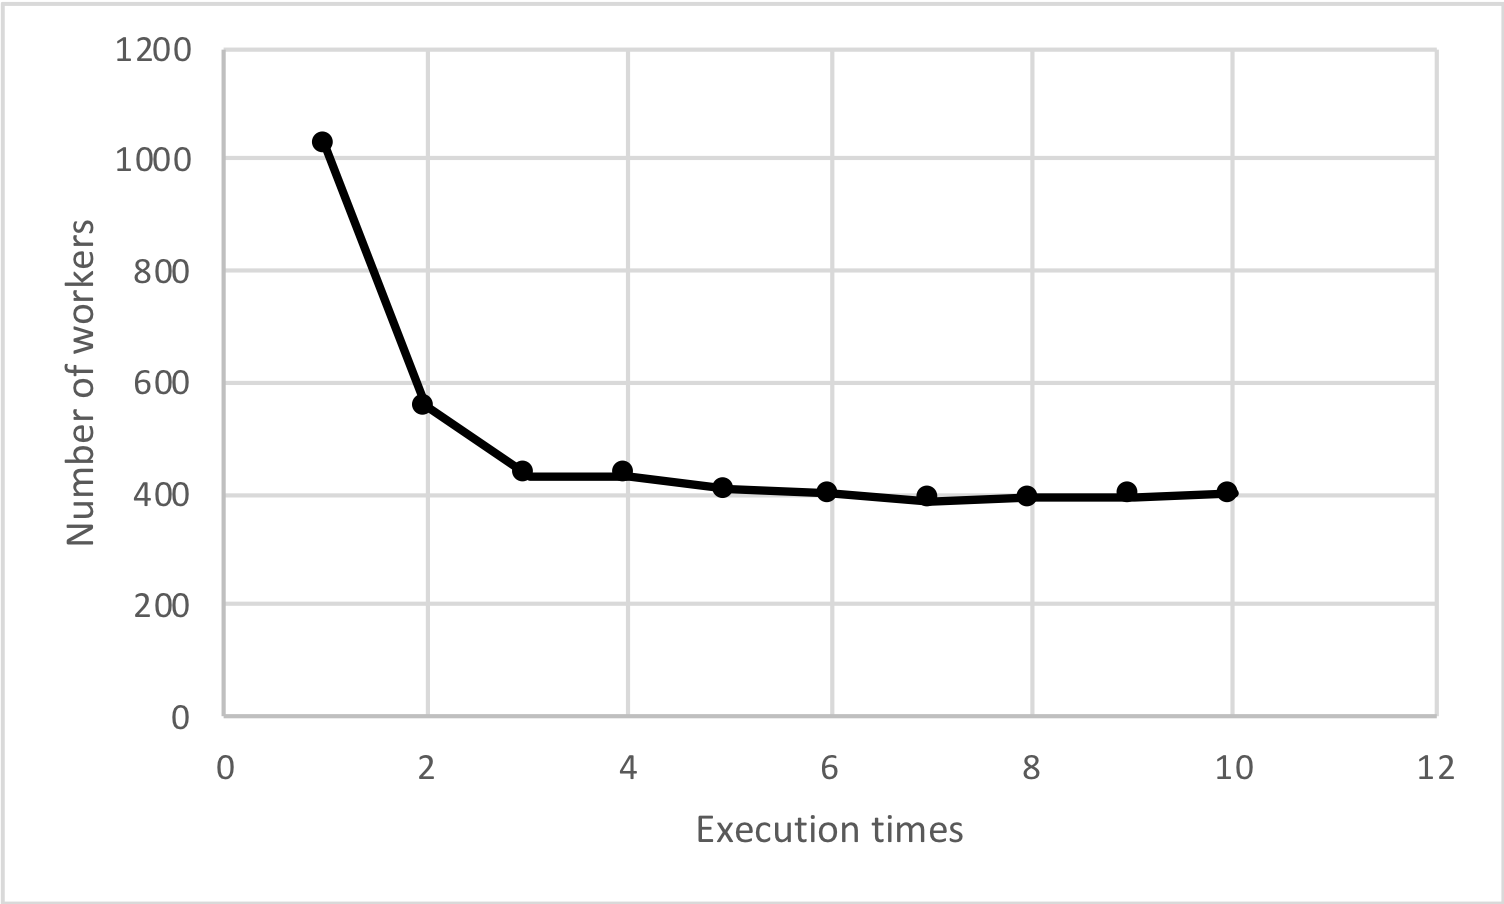
\includegraphics[width=\linewidth, height=\textheight, keepaspectratio]{res/execution_times.png}
    \caption{Grafico che mostra l'evoluzione dei tempi di esecuzione (in ms) al crescere del numero di worker. I tempi di esecuzione sono stati calcolati come media su 25 iterazioni considerando una schacchiera di gioco 5000x5000. I tempi di esecuzione sono stati calcolati su un Apple Macbook Pro (Retina, 15", metà 2015) dotato di un processore Intel Core i7 quad-core a 2.2GHz.}
    \label{fig:execution-times}
\end{figure}

\chapter{Esercizio 2 - Actor-based distributed chat}
\section{Analisi del problema}\label{analisi-del-problema-2}
Implementare una chat distribuita ad attori, con l'insieme dei partecipanti dinamico:
\begin{itemize}
    \item Un utente può aggiungersi e rimuoversi dinamicamente.
    \item Ogni messaggio inviato da un utente deve essere visualizzato da tutti gli altri utenti.
    \item Il sistema deve essere completamente decentralizzato.
        \begin{itemize}
            \item A parte, eventualmente, la presenza di un (attore) registro con indirizzo/nome noto che tenga traccia dei partecipanti.
        \end{itemize}
    \item I messaggi inviati nella chat devono essere visualizzati da tutti i partecipanti nel medesimo ordine.
\end{itemize}
Supporto per una modalità “sezione critica”:
\begin{itemize}
    \item Un partecipante può chiedere di entrare in sezione critica inserendo un comando predefinito (es: “:enter-cs”).
    \item Quando un partecipante entra in sezione critica, possono essere visualizzati solo i suoi messaggi, senza intervallarli a quelli degli altri utenti.
    \item Un solo partecipante alla volta può essere in sezione critica.
    \item Per uscire dalla sezione critica si può prevedere un altro comando predefinito (es: “:exit-cs”).
    \item Un utente può rimanere in sezione critica per un certo tempo massimo Tmax, dopodiché l’uscita è forzata.
    \item Durante una sezione critica i messaggi inviati dagli altri partecipanti devono essere rigettati.
\end{itemize}
\section{Descrizione della soluzione proposta}\label{soluzione-proposta-2}
\subsection{Architettura del sistema}\label{architettura-del-sistema-2}
Il sistema è stato organizzato utilizzando il modello ad attori. In particolare, gli attori presenti nella nostra soluzione sono due:
\begin{itemize}
    \item \texttt{User}: attore che si unisce alla stanza per partecipare alla chat distribuita.
    \item \texttt{Room}: attore centrale che funge da registro degli utenti presenti e inoltra i messaggi a tutti i partecipanti della chat.
    La \texttt{Room} gestisce anche la modalità 'sezione critica' della stanza.
\end{itemize}
\subsection{Dinamica del sistema}\label{dinamica-del-sistema-2}

La dinamica del sistema è stata rappresentata ad alto livello con un diagramma di sequenza, adatto per mostrare in modo efficace lo scambio di messaggi tra le entità del sistema.

Di seguito vengono mostrati i tre scenari d'interazione.

\begin{figure}[H]
    \centering
    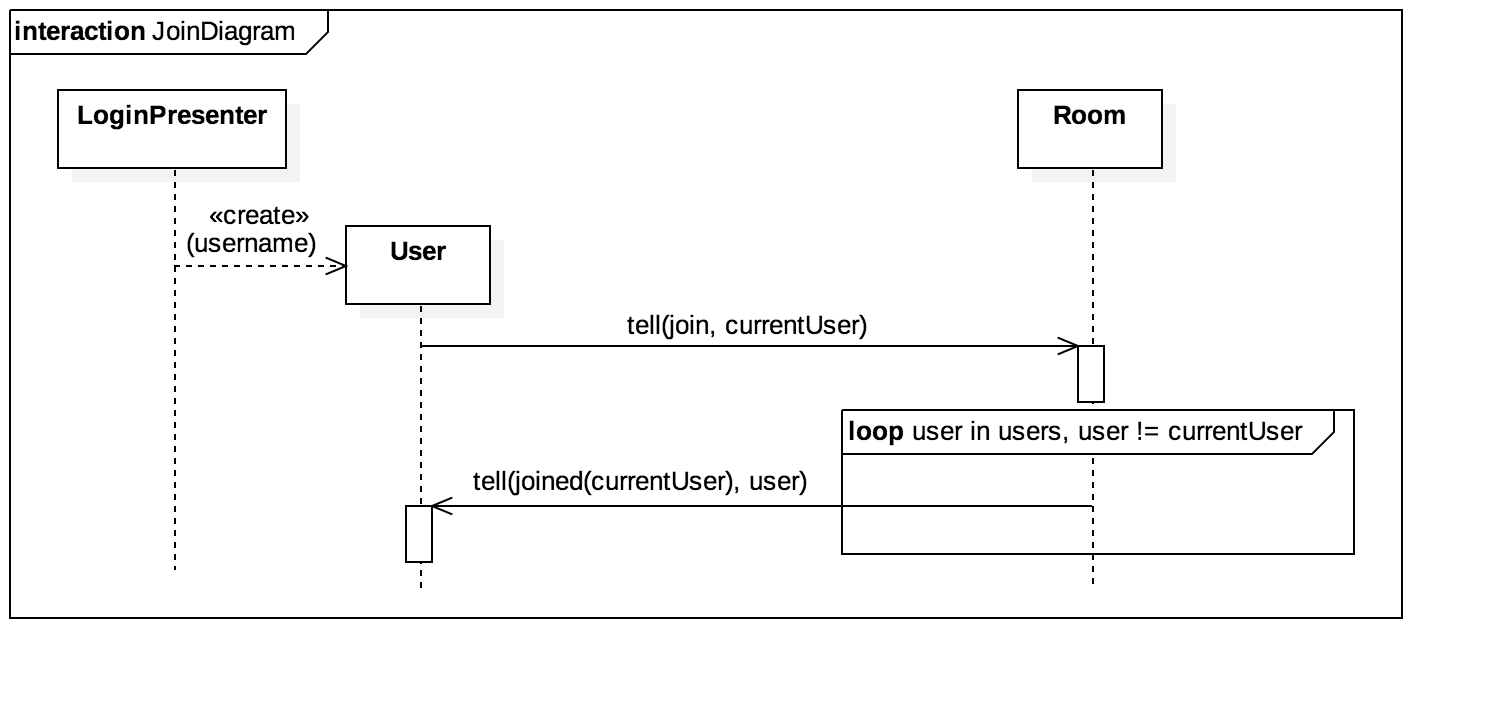
\includegraphics[width=\linewidth, height=\textheight, keepaspectratio]{res/JoinDiagram}
    \caption{Diagramma di sequenza che mostra l'unione di un utente alla stanza.}
    \label{fig:join-diagram}
\end{figure}

Nell'interazione descritta in figura \ref{fig:join-diagram} la sequenza di messaggi scambiati è la sequente:
\begin{enumerate*}[label=(\arabic*)]
%
    \item viene creato il nuovo utente;
%
    \item l'utente creato segnala alla stanza l'intenzione di volersi unire (join);
%
    \item la room segnala a tutti gli utenti presenti nella stanza l'aggiunta di un nuovo utente.
%
\end{enumerate*}

\begin{figure}[H]
    \centering
    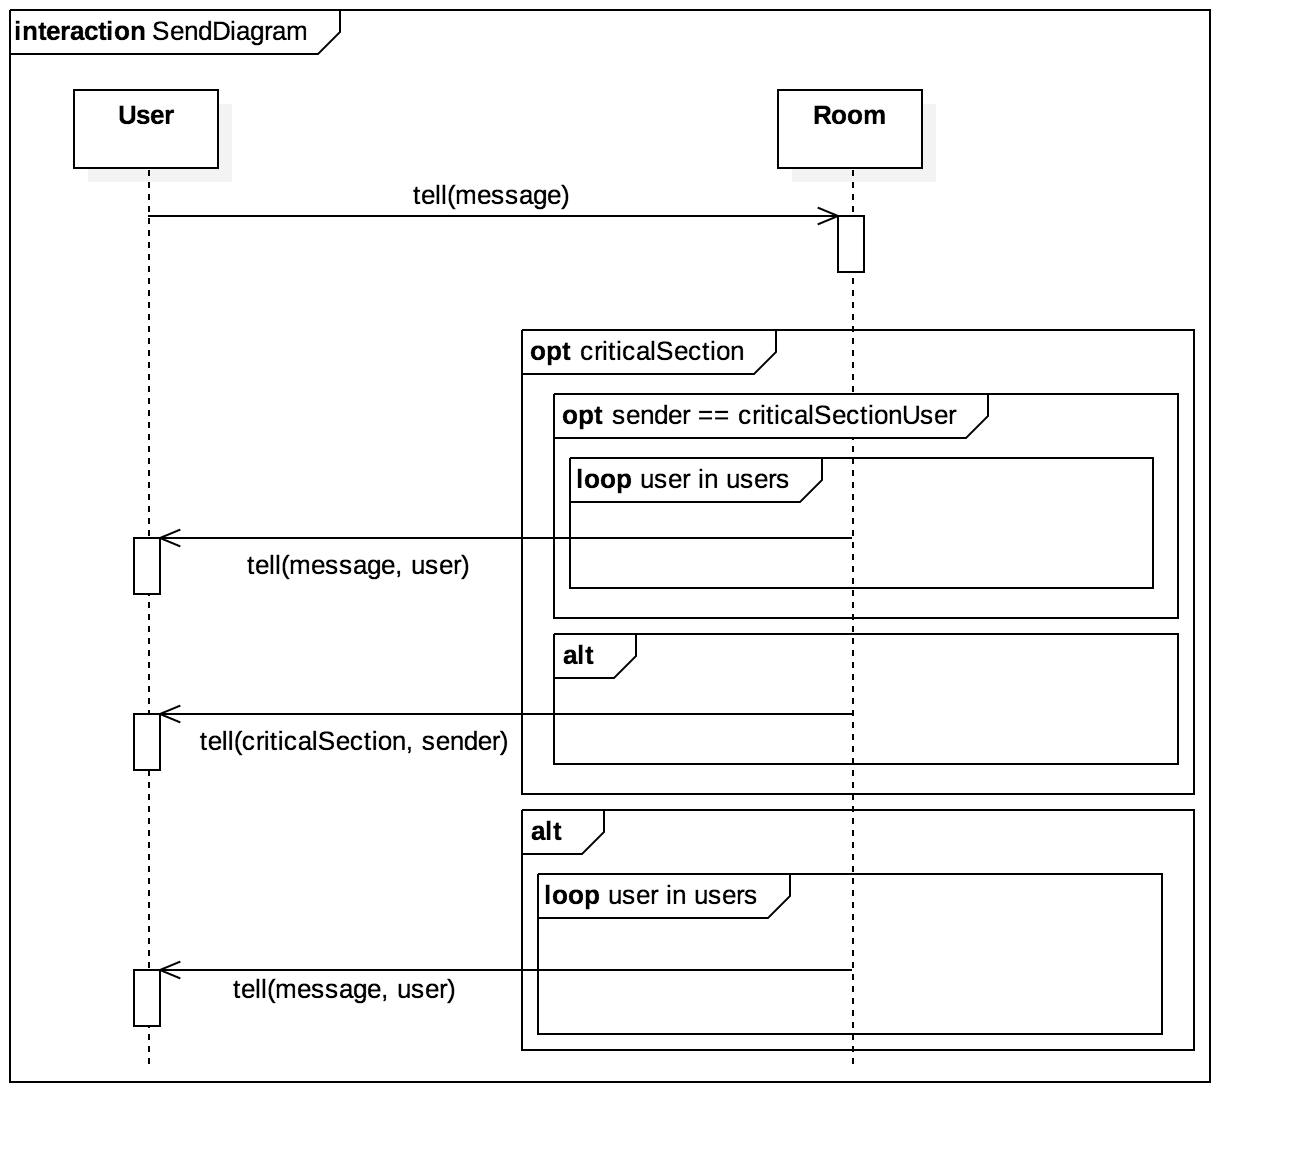
\includegraphics[width=\linewidth, height=\textheight, keepaspectratio]{res/SendDiagram}
        \caption{Diagramma di sequenza che mostra l'invio di un messaggio da parte di un utente al resto degli utenti presenti nella stanza.}
    \label{fig:send-diagram}
\end{figure}

Nell'interazione descritta in figura \ref{fig:send-diagram} la sequenza di messaggi scambiati è la sequente:
\begin{enumerate}[label=(\arabic*)]
%
    \item L'utente manda un messaggio alla room.
%
    \item Nel caso in cui ci sia una sezione critica:
        \begin{enumerate}
            \item se il mittente è l'utente in sezione critica il messaggio viene mandato a tutti gli altri;
%
            \item se il mittente non è l'utente in sezione critica, il messaggio viene rifiutato e viene segnalata al mittente l'identità dell'utente in sezione critica.
%
        \end{enumerate}
%
    \item Nel caso in cui non ci sia una sezione critica il messaggio viene inviato a tutti gli altri utenti.
\end{enumerate}

\begin{figure}[H]
    \centering
    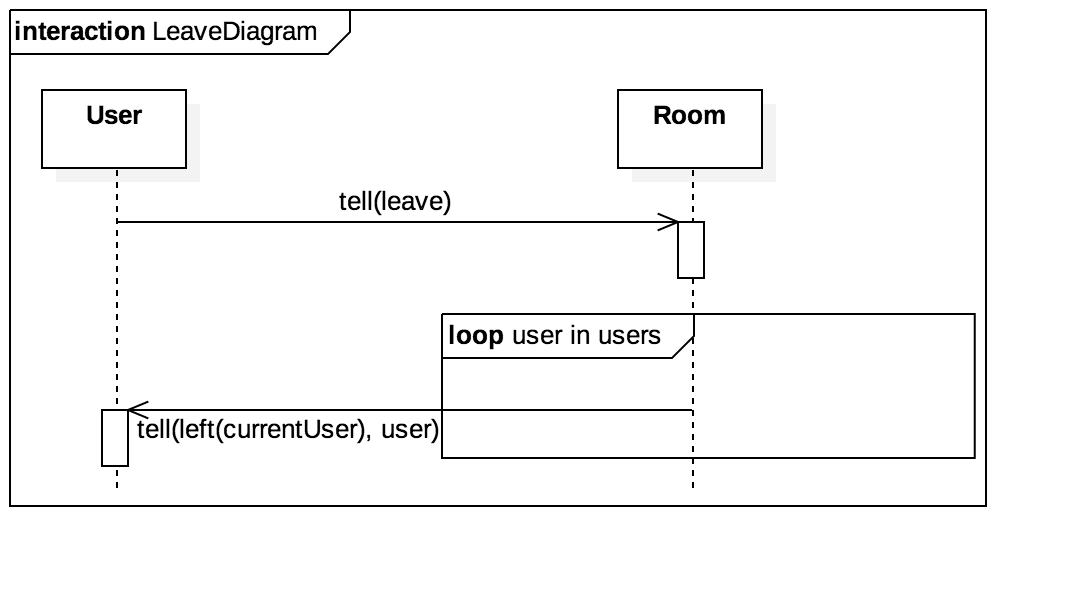
\includegraphics[width=\linewidth, height=\textheight, keepaspectratio]{res/LeaveDiagram}
        \caption{Diagramma di sequenza che mostra l'uscita di un utente dalla stanza.}
    \label{fig:leave-diagram}
\end{figure}

Nell'interazione descritta in figura \ref{fig:leave-diagram} la sequenza di messaggi scambiati è la sequente:
\begin{enumerate*}[label=(\arabic*)]
%
    \item l'utente segnala alla room che sta lasciando la stanza;
%
    \item la stanza segnala a tutti gli altri utenti l'identità dall'utente che ha lasciato la stanza.
%
\end{enumerate*}

\subsection{Algoritmo di ordinamento}\label{ordinamento-2}

Il problema dell'ordinamento dei messaggi può essere scomposto in due sottoproblemi tra loro indipendenti:

\begin{itemize}
%
    \item\textbf{causal message ordering}: assicura che tutti i messaggi vengano elaborati secondo il loro ordine di invio;
%
    \item\textbf{total message ordering}: assicura che tutti i processi elaborino i messaggi nello stesso ordine.
%
\end{itemize}

Il problema dell'ordinamento dei messaggi è stato risolto utilizzando due algoritmi che descriviamo di seguito. Questo permette ad ogni utente di avere una visione coerente e ordinata dei messaggi.

\subsection{Causal Message Ordering}\label{causal-message-ordering}

Ogni messaggio è costituito dal testo e dal numero di sequenza associatogli dal mittente.
Ogni utente mantiene per ogni processo il numero di messaggi inviati e viene aggiornato ogni volta che l'utente è abilitato a processare il messaggio ricevuto.\\
Un utente è abilitato ad elaborare il messaggio quando il numero di sequenza all'interno del messaggio è successivo al numero di sequenza dell'ultimo messaggio elaborato per quel mittente.
Se così non fosse, significa che ci sono dei messaggi precedenti del mittente che non sono ancora stati ricevuti ed è quindi necessario attendere il loro arrivo prima di potere elaborare il messaggio appena ricevuto.
\begin{enumerate}
    \item Un processo che si unisce al sistema riceve da tutti gli altri processi il loro numero di sequenza corrente.
    \item Un processo che invia un messaggio incrementa il proprio numero di sequenza e lo associa al messaggio.
    \item Un processo che riceve un messaggio controlla che il numero di sequenza contenuto nel messaggio sia successivo all'ultimo numero di sequenza che ha ricevuto dal mittente.\\
    Se tale condizione è soddisfatta:
    \begin{enumerate}
        \item il messaggio viene elaborato
        \item se ci sono altri messaggi che possono essere elaborati si ritorna al punto precedente.
    \end{enumerate}
    Se tale condizione non è soddisfatta il messaggio viene aggiunto alla coda dei messaggi in attesa.
    \item Un processo che esce dal sistema viene rimosso dalle liste di tutti gli altri processi.
\end{enumerate}

\subsection{Total Message Ordering}\label{total-message-ordering}

I processi inviano i messaggi al \textit{Sequencer}: entità che assegna un numero di sequenza globale ad ogni messaggio.
%Ogni processo memorizza il numero di sequenza globale dell'ultimo messaggio elaborato.
Ogni processo mantiene un contatore che rappresenta il numero di sequenza globale dell'ultimo messaggio elaborato.

Quando un utente invia un messaggio:
\begin{enumerate}
    \item Il \textit{Sequencer} assegna al messaggio un numero di sequenza.
    \item Un processo che riceve un messaggio controlla che il numero di sequenza del messaggio sia successivo all'ultimo numero di sequenza salvato.\\
    Se tale condizione è soddisfatta:
    \begin{enumerate}
        \item il messaggio viene elaborato
        \item se ci sono altri messaggi che possono essere elaborati si ritorna al punto precedente.
    \end{enumerate}
    Se tale condizione non è soddisfatta il messaggio viene aggiunto alla coda dei messaggi in attesa.
\end{enumerate}

\subsection{Implementazione}\label{implementazione-2}

%La soluzione è stata implementata utilizzando il linguaggio Scala e Akka come implementazione del modello ad attori.
La soluzione è stata implementata in linguaggio Scala utilizzando la libreria Akka. \`E stato scelto di utilizzare Scala e in particolare la libreria Akka perché permette di implementare gli attori in modo più agile e coinciso, evitando di scrivere \textit{boilerplate code}.\\
%Le entità presenti nel sistema sono gli utenti della chat (un utente è rappresentato dall'attore \texttt{User}) e una stanza, utilizzata dagli utenti per comunicare tra loro, che funge da registro e da coordinatore (rappresentata dall'attore \texttt{Room}).
Le entità presenti nel sistema sono gli utenti della chat (rappresentati dall'attore \texttt{User}) e un sistema che funge da registro e da coordinatore (rappresentato dall'attore \texttt{Room}).

\subsubsection{Dettaglio d'interazione}
\paragraph{Join}
L'utente che si unisce alla stanza invia a quest'ultima un messaggio di \texttt{Join}; tale messaggio viene inviato durante l'esecuzione del metodo \texttt{preStart()} del ciclo di vita di un attore Akka.
Alla ricezione di tale messaggio la stanza informa gli utenti dell'arrivo del nuovo utente (\texttt{Joined(user)}) e risponde a quest'ultimo con il numero di sequenza globale della stanza (che d'ora in poi chiameremo $s_g$).
Gli altri utenti, informati dalla stanza, inviano al nuovo utente il loro personale numero di sequenza (relativo al numero di messaggi da loro inviati, che d'ora in poi chiameremo $s_{u_i}$) affinché possa aggiungerlo ad una lista. Questo permette al nuovo utente di sincronizzarsi con gli altri utenti, così da poter elaborare d'ora in avanti i messaggi scambiati.
Infine la stanza aggiunge il nuovo utente alla lista degli utenti presenti nel sistema.

\paragraph{Messages}
Quando un utente $i$ intende inviare un messaggio prima chiede alla stanza se è in sezione critica. Se la stanza non è in sezione critica incrementa $s_{u_i}$ e poi lo allega al messaggio (\texttt{Message(content, user, userCounter)}).
Altrimenti nel caso l'utente detenga la sezione critica, allora può inviare il messaggio come descritto nel punto precedente. Nel caso in cui sia detenuta da qualcun altro non può inviare il messaggio.
La stanza, alla ricezione del messaggio, incrementa $s_g$ ed inoltra a tutti gli utenti del sistema il messaggio allegandogli $s_g$.
\\~\\
Ogni utente, alla ricezione del messaggio inviatogli dalla stanza, controlla che $s_g$ contenuto nel messaggio sia successivo all'$s_g$ dell'ultimo messaggio elaborato. Se così fosse, è possibile passare al controllo dell'ordine causale che consiste nel verificare che il numero di sequenza $s_{u_i}$ contenuto nel messaggio sia successivo al $s_{u_i}$ dell'ultimo messaggio eleborato che è stato inviato dall'utente $i$.

\paragraph{EnterCriticalSection \& ExitCriticalSection}
Per entrare in sezione critica, un utente invia il messaggio \texttt{EnterCriticalSection} alla stanza. La sezione critica può essere acquisita solo se non è detenuta da qualche altro utente, in tal caso il richiedente acquisisce la sezione critica e solo lui potrà inviare messaggi.

Per uscire dalla sezione critica, l'utente che la detiene dovrà inviare il messaggio \texttt{ExitCriticalSection}. A questo punto la stanza informa tutti gli utenti che la sezione critica è stata rilasciata.

\paragraph{Leave}
Quando un utente esce dal sistema, viene chiamato il metodo del ciclo di vita di un attore Akka \texttt{postStop()}, il quale invia un messaggio \texttt{Leave} alla stanza. Quest'ultima informa tutti gli altri utenti dell'uscita dell'utente, così sia la stanza sia gli utenti possono rimuoverlo dalla lista.

\subsubsection{Interfaccia grafica}
L'interfaccia grafica è stata realizzata utilizzando ScalaFX: una libreria che wrappa le funzionalità di JavaFX fornendole in stile funzionale.
All'interno del sistema sono presenti due schermate principali: una per il login e una per la chat.\\
Per ogni vista è presente un'apposita classe con suffisso \texttt{View} che ne definisce i componenti grafici e una classe con suffisso \texttt{Presenter} che gestisce gli eventi ad essa associati.
La \texttt{ChatView} al momento della sua inizializzazione si preoccupa di mettere in esecuzione il sistema degli Attori, mentre il relativo \texttt{ChatPresenter} mantiene il riferimento all'attore che modella l'utente per gestire le interazioni nel sistema a seguito degli eventi scatenati nell'interfaccia e viceversa.

\newpage

\appendix
\section{Comandi}
I comandi inviabili alla stanza sono:
\begin{itemize}
    \item \textit{:enter-cs}: per richiedere l'entrata in sezione critica da parte di un utente
    \item \textit{:exit-cs}: per richiedere l'uscita dalla sezione critica da parte di un utente
    \item \textit{:help}: per richiedere la lista dei comandi disponibili
\end{itemize}

% Your document ends here!
\end{document}
